\documentclass[10pt]{article}
\usepackage[a4paper,margin=2cm]{geometry}
\usepackage{amsmath}
\usepackage{booktabs}
\usepackage{longtable}
\usepackage{array}
\usepackage{xcolor}
\usepackage{colortbl}
\usepackage{fancyvrb}
\usepackage{titlesec}
\usepackage{enumitem}
\usepackage{hyperref}
\usepackage{graphicx}
\hypersetup{colorlinks=true,linkcolor=blue!50!black,urlcolor=blue!50!black}
\titlespacing*{\section}{0pt}{1.2ex}{0.6ex}
\titlespacing*{\subsection}{0pt}{0.9ex}{0.4ex}
\setlist{nosep,leftmargin=1.4em}
\definecolor{fire}{RGB}{225,245,225}
\definecolor{neg}{RGB}{250,225,225}
\definecolor{hdr}{RGB}{235,235,240}
\newcommand{\cmd}[1]{\texttt{\small #1}}

\title{\vspace{-1.5cm}\textbf{ScienceWorld: environment inspection report}\\[2pt]
\large Wave-0 M5, CA-Benchmark project}
\author{}
\date{2026-07-23}

\begin{document}
\maketitle
\vspace{-0.6cm}

\noindent\small\textit{Scope.} Hands-on inspection of the ScienceWorld text environment (rung~4 of
the credit-assignment benchmark): what the tasks are, how they are scored and evaluated, how many
trials exist, rollout speed on our node, the sandbox/action surface, a full worked trajectory, expert-data
availability, published baselines, and the challenges that bear on training. All local numbers are
reproduced by \cmd{scripts/scienceworld/audit\_structure.py}, \cmd{analyze\_audit.py}, and
\cmd{bench\_and\_probe.py}; raw assets are in \cmd{assets/}. Package: \cmd{scienceworld 1.2.3} (pip) on
OpenJDK~17, one CPU worker.\normalsize

\section{What the environment is (the sandbox)}
ScienceWorld (Wang et al., EMNLP 2022; arXiv 2203.07540) is a \textbf{text-based interactive simulator of
elementary-school science}. The agent navigates a map of \textbf{10 locations} centered on a house
(hallway, kitchen, bathroom, workshop, art studio, greenhouse, bedroom, living room, foundry, outside/
garden), populated with \textbf{up to 200 object types}, carrying out science procedures. It is
\textbf{partially observable}: \cmd{look around} reveals only the current room; the underlying engine
tracks a full thermodynamic / chemical / biological state (temperatures, states of matter, electrical
circuits, plant and animal life-cycles) that the agent must actively probe with instruments.

\smallskip
\noindent\textbf{Engine \& interface.} The simulator core is \textbf{$\sim$40k lines of Scala}
(compiled to a JAR, run on Java 1.8+) exposed to Python via \texttt{py4j} --- a JVM must be present (we
installed OpenJDK~17). Verified from the source: each \cmd{ScienceWorldEnv} launches \textbf{its own
dedicated JVM process} (plus a Python callback server); there is no documented thread-safety mechanism, so
\textbf{parallelism is process-level} (the paper's RL runs used 8 parallel env instances). For us this
means the environment is CPU/JVM-bound and single-threaded per instance; worker throughput scales with the
number of env processes we co-locate with the trainer, not with threads.

\smallskip
\noindent\textbf{Action space (25 templates).} Actions are \emph{template + object(s)} combinations:

\begin{center}\small
\begin{tabular}{lll}
\cmd{activate/deactivate OBJ} & \cmd{open/close OBJ} & \cmd{focus on OBJ} \\
\cmd{go OBJ} & \cmd{teleport OBJ} & \cmd{look around / look at / look in OBJ} \\
\cmd{pick up / put down OBJ} & \cmd{move OBJ to OBJ} & \cmd{pour OBJ in OBJ} \\
\cmd{dunk OBJ in OBJ} & \cmd{mix OBJ} & \cmd{use OBJ on OBJ} \\
\cmd{read OBJ} & \cmd{eat OBJ} & \cmd{flush OBJ} \\
\cmd{wait / wait1} & \cmd{inventory} & \cmd{task} \\
\end{tabular}
\end{center}

\noindent The \textbf{combinatorial action space} is the headline difficulty: the paper estimates
\textbf{$\approx$200{,}000 naively-possible action--object combinations per step}; in our own probe a
single \cmd{boil} start-state already exposes \textbf{115 valid combinations}, growing as the agent
uncovers objects. A free-text agent (our ReAct policy) is \emph{not} handed this list --- it must generate
a valid \cmd{Thought:/Action:} string, and malformed or inapplicable actions get a soft error observation
(e.g.\ \cmd{"You can't move something into itself."}). Critically, the paper reports that all but two of
its baselines relied on a \textbf{valid-action-detection aid} at test time to shrink this search --- a
crutch our generative agent does not use, which makes valid-action-rate a first-class diagnostic.
\textbf{Simplifications} can be toggled; the audit used the standard \cmd{easy} set (\cmd{teleportAction},
\cmd{openDoors}, \cmd{selfWateringFlowerPots}, \cmd{noElectricalAction}) --- these must be frozen
identically across all arms and recorded, since they change both horizon and answerability.

\section{The tasks and how they are scored (the evaluation)}
There are \textbf{30 tasks} (10 topic categories) spanning thermodynamics, chemistry/mixing, electricity,
classification, biology (life stages, lifespans, plant growth, genetics), and measurement; we group them
into \textbf{10 families} (\cmd{assets/families.csv}). The paper reports \textbf{7{,}200 total variations
across all 30 tasks} --- different target substances, objects, and layouts. Each task ships fixed
\textbf{train / dev / test} variation splits ($\approx$50/25/25\%), so ``unseen variations'' is a
built-in generalization split --- no custom splitting needed. The original protocol resets an episode at
success, failure, or a \textbf{100-step cap}; we replace that single global cap with per-family caps
(below), since horizons range $\sim$40$\times$.

\smallskip
\noindent\textbf{Scoring is a dense, cumulative 0--100 subgoal score.} The per-step \texttt{reward}
returned by the API is the score \emph{delta}. From replaying 90 gold trajectories (3 train variations
$\times$ 30 tasks):
\begin{itemize}
\item All 90 gold paths reach exactly \textbf{score 100 with \texttt{done}=True}; no negative deltas on-path.
\item Subgoal firing density: median \textbf{0.27} score-increments per step (range 0.05--0.62) --- dense
relative to a terminal-only signal, but far from every-step.
\item \textbf{Magnitudes are heterogeneous and task-specific: 42 distinct values from 1 to 72.} The oracle
is \emph{not} a uniform unit-per-subgoal reward. Any process-reward (PRM) arm in the side experiments must
match this granularity or renormalize explicitly and say so.
\item \textbf{Off-gold failure is catastrophic:} a wrong \cmd{focus on} (focusing on the wrong object)
returns \textbf{reward $-100$ and immediately terminates the episode}. \cmd{focus} is thus both a hard
subgoal gate and an instant-death / reward-hacking surface for exploration.
\end{itemize}

\noindent\textbf{Our reward convention (proposed, confirm at W1 manifest).} Core-matrix arms train on
\emph{terminal success only}: success $\Leftrightarrow$ final score $=100$; a $-100$ focus-death maps to
terminal reward $0$ and episode end (mirroring ALFWorld failure, keeping terminal reward in $\{0,1\}$).
The dense 0--100 oracle is reserved for the PRM-ladder / redistribution side experiments, where the $-100$
event is exactly the kind of asymmetry the redistribution-vs-separation question probes.

\smallskip
\noindent\textbf{Oracle isolation (checked).} Observation text on all 90 gold paths contained zero
\cmd{score}/\cmd{reward}/\cmd{subgoal}/\cmd{points} strings; the score lives only in the API \texttt{info}
dict, and the \cmd{task} command exposes only the task description (already in the prompt). So a
transcript-only agent is blind to the oracle --- a prerequisite for the "rubric PRM must not see oracle
state" guarantee. (One residual: audit our own env \emph{wrapper} once written.)

\section{How many trials, and rollout speed}
\textbf{Trials.} 30 tasks with widely varying variation counts --- from \textbf{4} train variations
(\cmd{identify-life-stages-2}) to \textbf{692} (\cmd{inclined-plane-friction-named-surfaces}). The
\cmd{find-*} and \cmd{test-conductivity} families have 150--450 train variations each. The paper's
\textbf{7{,}200 total variations} (train+dev+test across all tasks) means that, unlike a fixed-size QA
set, ScienceWorld supplies a large pool of fresh task instances --- the training-time question is the
\emph{sampling} policy (uniform-per-task vs uniform-per-variation), which we must fix before Wave~1 because
the 4-vs-692 imbalance changes what one ``epoch'' means and which tasks dominate the gradient.

\smallskip
\noindent\textbf{Rollout speed} (single JVM env, our node; \cmd{assets/speed\_bench.json}):
\begin{center}\small
\begin{tabular}{lr}
\toprule
Operation & measured \\
\midrule
\cmd{load(task,var)} + \cmd{reset} & 0.22 s/episode (0.15--0.36) \\
Gold-action stepping & \textbf{13.8 steps/s} (73 ms/step) \\
Random stepping, \cmd{step} only & 15.3 steps/s (65 ms/step) \\
Random stepping incl.\ \cmd{get\_valid\_actions} each step & 9.0 steps/s (112 ms/step) \\
\bottomrule
\end{tabular}
\end{center}

\noindent\textbf{Reading for training budget.} At $\approx$65--75 ms/env-step, one env instance yields
$\sim$14 steps/s. The horizon is the multiplier that matters: a 30-step task costs $\sim$2 s of pure env
time, but a 200-step \cmd{inclined-plane} episode costs $\sim$14 s \emph{of CPU env time alone}, before any
LLM generation. This is why ScienceWorld is the most expensive rung per environment-episode and why
long-horizon families dominate wall-clock. Querying the valid-action set every step (which we do
\emph{not} need for a free-text agent) nearly halves throughput --- keep it out of the hot loop. Env
parallelism is process-level (one JVM each), so worker-level throughput scales with the number of env
workers we run alongside the trainer.

\section{A full trajectory (gold/expert)}
\textbf{Expert data is available for free:} the engine generates a \textbf{gold action sequence} for any
task/variation (\cmd{generateGoldPath=True} $\rightarrow$ \cmd{get\_gold\_action\_sequence()}). This is our
rung-4 SFT/$\pi_\text{base}$ source (rendered into the ReAct grammar, with the score channel stripped ---
oracle isolation). No external expert dataset is needed. Below is a complete gold trajectory for a short
task; green rows mark subgoal firings (with the reward increment), showing how the dense signal is
distributed along the path.

\smallskip
\noindent\textbf{Task \cmd{find-animal} (variation 0), 10 gold steps, final score 100.}\\
\textit{"Your task is to find a(n) animal. First, focus on the thing. Then, move it to the red box in the kitchen."}
\begin{center}\small
\begin{tabular}{r>{\raggedright\arraybackslash}p{5.2cm}>{\raggedright\arraybackslash}p{6.5cm}r}
\rowcolor{hdr}\hline
$t$ & action & observation & $\Delta$score \\ \hline
0 & \cmd{open door to greenhouse} & The door is already open. & \cellcolor{fire}+8 \\
1 & \cmd{go to greenhouse} & You move to the greenhouse. & \cellcolor{fire}+9 \\
2 & \cmd{open door to outside} & The door is already open. & \\
3 & \cmd{go to outside} & You move to the outside. & \\
4 & \cmd{look around} & \dots an axe, a blue jay egg, \dots (many objects) & \\
5 & \cmd{focus on blue jay egg} & You focus on the blue jay egg. & \cellcolor{fire}+50 \\
6 & \cmd{pick up blue jay egg} & You move the blue jay to the inventory. & \cellcolor{fire}+8 \\
7 & \cmd{open door to kitchen} & The door is already open. & \\
8 & \cmd{go to kitchen} & You move to the kitchen. & \cellcolor{fire}+8 \\
9 & \cmd{move blue jay egg to red box} & You move the blue jay to the red box. & \cellcolor{fire}+17 \\ \hline
\end{tabular}
\end{center}

\noindent A second, richer trajectory (\cmd{change-the-state-of-matter-of} water, 22 steps, in
\cmd{assets/full\_traj\_*.json}) shows the harder physics: the agent picks up a thermometer, puts water in
a metal pot, \cmd{focus on substance in metal pot} (\textbf{+66}, the big subgoal gate), moves it to the
freezer (+2), then \cmd{wait}s while probing temperature (10\,\textdegree C $\rightarrow$ 3\,\textdegree C)
until the water freezes and the final \cmd{wait} fires \textbf{+29} to reach 100. It illustrates three
training-relevant traits at once: \textbf{partial observability} (state read only via the thermometer),
\textbf{delayed physical dynamics} (must \cmd{wait} for freezing --- reward arrives many steps after the
causal action), and \textbf{a dominant single subgoal} (\cmd{focus} worth 66/100), which shapes what credit
assignment has to discover.

\section{Published baselines (original paper + follow-ups)}
\textbf{Original paper (Table 2; test variations; 0--1 scale).} The headline finding is that
\emph{elementary science is hard for text agents and larger models are not better}: a 1.5M-parameter RL
agent trained interactively for 100k steps beats an 11B model trained statically for science QA.

\begin{center}\small
\begin{tabular}{lrr}
\toprule
Agent & Params & Avg score (0--1) \\
\midrule
Random-valid & --- & 0.03 \\
\textbf{DRRN} (best baseline) & 1.5M & \textbf{0.17} \\
KG-A2C & 5.5M & 0.11 \\
CALM (GPT-2) & 131M & 0.05 \\
Behavior Cloning (T5-11B) & 11B & 0.08 \\
Text Decision Transformer (T5-11B) & 11B & 0.08 \\
\bottomrule
\end{tabular}
\end{center}
\noindent\footnotesize Best agent 0.17/1.0 --- comparable to text agents on medium-difficulty
interactive-fiction games. The paper notes all but two baselines leaned on the valid-action aid at test
time. Source: arXiv 2203.07540 Table 2.\normalsize

\smallskip
\noindent\textbf{Follow-ups (0--100 scale; note the differing eval sets --- not directly comparable across
rows).} Modern LLM agents changed the picture dramatically:
\begin{center}\small
\begin{tabular}{lllr}
\toprule
Method & Base model & Eval set & Avg score \\
\midrule
DRRN / KG-A2C / CALM & (paper baselines) & 270 test vars & 15.6 / 11.4 / 5.1 \\
SayCan & GPT-4 & 270 test vars & 33.8 \\
ReAct & GPT-4 & 270 test vars & 36.4 \\
Reflexion & GPT-4 & 270 test vars & 45.3 \\
\textbf{SwiftSage} & T5-large (770M) + GPT-4 & 270 test vars & \textbf{84.7} \\
\midrule
PPO & Llama-2-7B-Chat & 194 seen / 241 unseen & 59.4 / 51.7 \\
SFT & Llama-2-7B-Chat & 194 seen / 241 unseen & 67.4 / 53.0 \\
\textbf{ETO} & Llama-2-7B-Chat & 194 seen / 241 unseen & \textbf{73.8 / 65.0} \\
GPT-4 (ETO paper) & GPT-4 & 194 seen / 241 unseen & 64.8 / 64.4 \\
\midrule
BC-large & Llama-2-7B-Chat & AgentGym split & 74.5 \\
AgentEvol & Llama-2-7B-Chat & AgentGym split & 38.0 \\
GPT-4-Turbo (AgentGym) & GPT-4-Turbo & AgentGym split & 14.4 \\
\bottomrule
\end{tabular}
\end{center}
\noindent\footnotesize Sources: SwiftSage arXiv 2305.17390 (first 10 test variations/task = 270);
ETO arXiv 2403.02502 / ACL 2024 (avg reward, seen/unseen); AgentGym arXiv 2406.04151.
\textbf{Reading for us:} (1) a 7B open model with the right training (ETO 65--74, SFT 53--67) is a
realistic target band for our Qwen3-4B rung-4 numbers --- meaning 4B \emph{can} get off the ground here,
unlike the ASearcher worry. (2) SFT/BC is a \emph{very} strong baseline on this env (BC-large 74.5,
SFT-seen 67.4), so our SFT $\pi_\text{base}$ floor rows matter enormously --- an RL arm must clear a high
bar, and AgentEvol \emph{losing} to BC-large is a cautionary precedent. (3) The GiGPO/verl-agent and
RAGEN lineages do \textbf{not} report ScienceWorld, so our rung-4 numbers are largely new territory for
those exact methods --- good for novelty, but no in-method reference point exists. \textbf{Caveat:} every
follow-up uses a different eval subset (270 vs 194/241 vs AgentGym), so cross-row comparison is
illustrative only; our SOTA table (§10 of the overview) will carry base-model + split + metric columns to
avoid the mismatched-settings trap.\normalsize

\section{Challenges (why this rung matters for credit assignment)}
\begin{enumerate}
\item \textbf{Long, variable horizons (5--200+ steps).} Sampled gold-path lengths span $\sim$40$\times$
within one rung (see per-family table), giving RQ2 within-rung horizon strata for free --- but also making
this the hardest rung for flat trajectory-level credit, which is exactly the hypothesis under test.
\item \textbf{Combinatorial action space} ($>$100 valid combos/step) with soft failure on invalid actions
--- a free-text agent must \emph{generate} legal actions, so a valid-action-rate metric is a leading
diagnostic (as it was in the ALFWorld pilot).
\item \textbf{Partial observability + delayed dynamics.} Rewarding actions (focus, heat, wait) often pay
off many steps later, and world state must be actively measured. This is the regime where a turn-level
critic or anchor-state advantage should, in principle, beat token-broadcast GRPO.
\item \textbf{Catastrophic \cmd{focus} death ($-100$, instant end).} A per-turn hacking/instant-fail
surface; needs a focus-death-rate counter and a decided terminal mapping.
\item \textbf{Heterogeneous dense reward (magnitudes 1--72, one subgoal often dominates).} Makes the naive
``sum dense + terminal'' channel spiky --- the motivation for the redistribution-vs-separation side
experiment.
\item \textbf{Context blow-up on long families.} Proposed 2$\times$-gold turn caps reach 260--404 for
genetics / matter-state / inclined-plane; full-history transcripts will not fit at 4B, so oldest-observation
truncation is load-bearing for 4 of 10 families. Final caps await strong-model turns-to-success calibration.
\item \textbf{Task-sampling / variation imbalance (4 vs 692 variations).} Must be fixed a priori so
``epoch'' and the train/unseen generalization gap are well-defined.
\end{enumerate}

\section*{Per-family horizons and proposed turn caps}
\begin{center}\small
\begin{tabular}{lrr}
\toprule
family & sampled gold-len range & proposed cap ($2\times$max) \\
\midrule
lifespan & 6--9 & 18 \\
find-thing & 5--16 & 32 \\
chemistry-mix & 11--30 & 60 \\
life-stages & 10--30 & 60 \\
electricity & 9--45 & 90 \\
plant-growth & 66--85 & 170 \\
thermal-measure & 18--94 & 188 \\
genetics & 123--130 & 260 \\
matter-state & 20--143 & 286 \\
inclined-plane & 53--202 & 404 \\
\bottomrule
\end{tabular}
\end{center}
\noindent\footnotesize Caps are provisional (2$\times$ the longest sampled gold path); they will be
finalized from strong-model (gpt-oss-120b) rollout turns-to-success (95th percentile) rather than the gold
heuristic alone, since gold paths contain filler an agent may skip or exceed. Annotated HTML trajectories
in \cmd{assets/html/}.\normalsize

\begin{center}
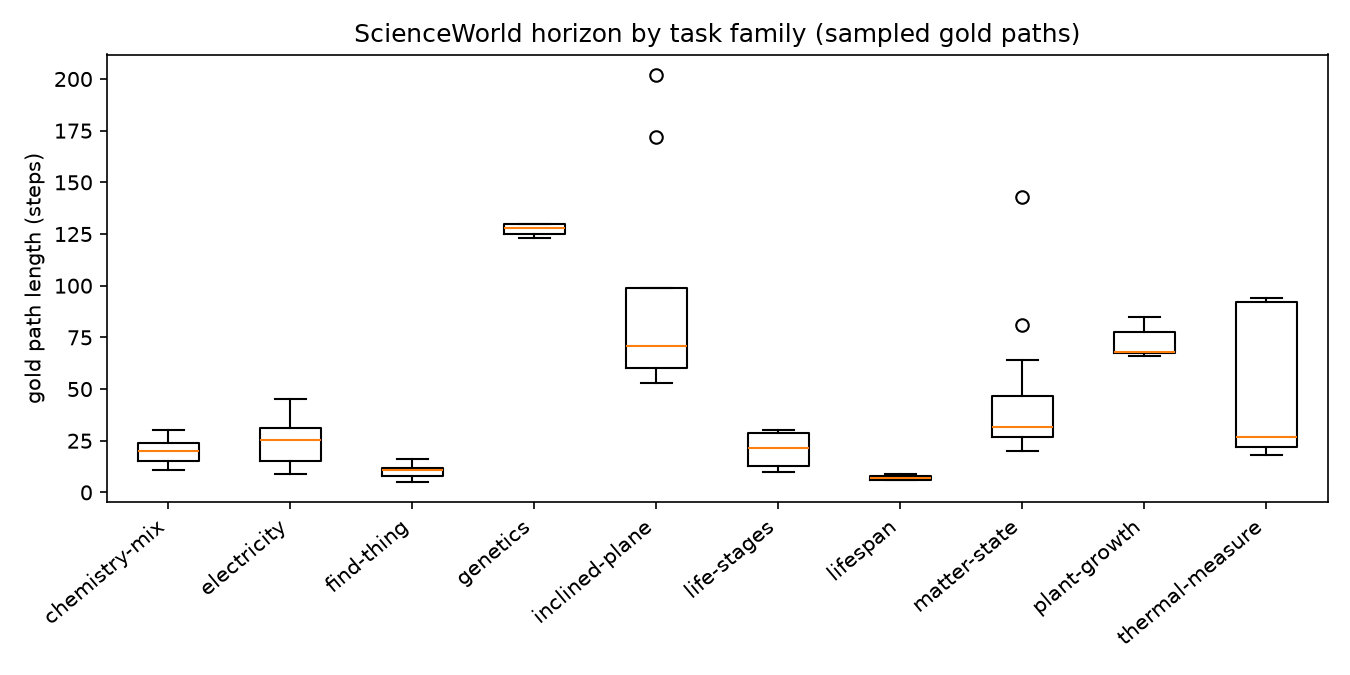
\includegraphics[width=0.82\textwidth]{horizon_hist.png}
\end{center}
\vspace{-0.4cm}
\noindent\footnotesize\textit{Gold-path length (steps) by task family, 3 sampled train variations each ---
the $\sim$40$\times$ within-rung horizon spread that gives RQ2 its horizon strata.}\normalsize

\end{document}
